\documentclass[11pt, a4paper]{article}

% --- Packages ---
\usepackage[utf8]{inputenc}
\usepackage[T1]{fontenc}
\usepackage{geometry}
\geometry{margin=1in}
\usepackage{hyperref}
\usepackage{listings}
\usepackage{xcolor}
\usepackage{booktabs}
\usepackage{graphicx}
\usepackage{amsmath}
\usepackage{caption}
\usepackage{float}
\usepackage{enumitem}
\usepackage{graphicx}
% --- Code Block Styling ---
\definecolor{codegray}{rgb}{0.5,0.5,0.5}
\definecolor{backcolour}{rgb}{0.96,0.96,0.94}
\definecolor{codeblue}{rgb}{0.1, 0.2, 0.6}

\lstset{
	backgroundcolor=\color{backcolour},
	basicstyle=\ttfamily\small,
	keywordstyle=\color{codeblue},
	breaklines=true,
	captionpos=b,
	keepspaces=true,
	numbers=left,
	numbersep=5pt,
	numberstyle=\tiny\color{codegray},
	showspaces=false,
	showstringspaces=false,
	frame=single,
	rulecolor=\color{black!30}
}

% --- Document Information ---
\title{\textbf{Multi-Container Runtime with Kernel Memory Monitor}}
\author{
	\textbf{S. Kishore} (PES1UG24CS607) \\
	\textbf{Darshan Doddamani} (PES1UG24CS566)
}
\date{}

\begin{document}
	
	\maketitle
	
	\hrule
	\vspace{0.5cm}
	
	\section{Introduction}
	This project implements a custom container runtime environment featuring a user-space supervisor and a specialized Linux kernel module for real-time memory monitoring and enforcement. The system provides process isolation via Linux namespaces and manages container lifecycles through a centralized engine.
	
	\section{Build and Setup Instructions}
	
	\subsection{Prerequisites}
	The implementation is designed for \textbf{Ubuntu 22.04/24.04} environments. It requires kernel headers for module compilation and \textbf{Secure Boot} must be disabled to load the custom kernel module.
	
	\begin{lstlisting}[language=bash]
		sudo apt update
		sudo apt install -y build-essential linux-headers-$(uname -r)
	\end{lstlisting}
	
	\subsection{Build and Load}
	The project uses a structured \texttt{Makefile} to compile the supervisor, kernel monitor, and test workloads simultaneously.
	
	\begin{lstlisting}[language=bash]
		# Build all components
		make -C boilerplate
		
		# Load the kernel monitor
		sudo insmod boilerplate/monitor.ko
	\end{lstlisting}
	
	\section{System Architecture \& Demo Demos}
	
	\subsection{Multi-Container Supervision}
	The supervisor process creates isolated environments using \texttt{clone()} with \texttt{CLONE\_NEWPID}, \texttt{CLONE\_NEWNS}, \texttt{CLONE\_NEWUTS}, and \texttt{CLONE\_NEWNET} flags.
	
	\begin{figure}[H]
		\centering
		 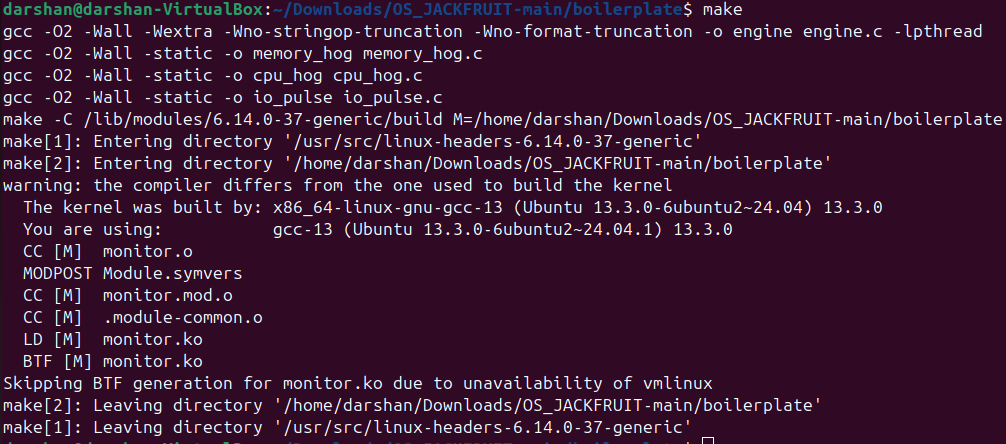
\includegraphics[width=0.85\textwidth]{screenshots/1.png}
		\caption{Demo 1: Concurrent execution of 'alpha' and 'beta' containers.}
	\end{figure}
	
	\subsection{Metadata and State Tracking}
	The supervisor tracks the state of every container, including its PID, memory limits, and scheduling priority (nice value).
	
	\begin{figure}[H]
		\centering
		 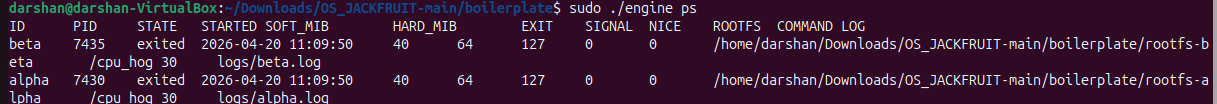
\includegraphics[width=0.85\textwidth]{screenshots/2.png}
		\caption{Demo 2: Metadata tracking via 'ps' command output.}
	\end{figure}
	
	\subsection{Logging Pipeline}
	Logs are managed via a bounded-buffer producer/consumer model. Producers read from container pipes and a single logger thread flushes data to per-container files.
	
	\begin{figure}[H]
		\centering
		 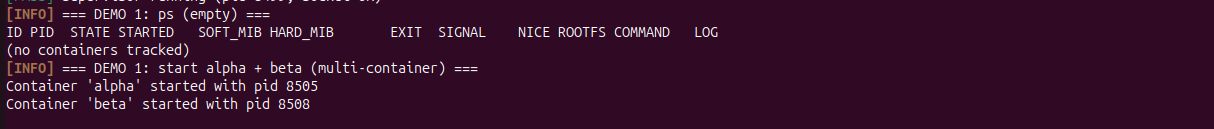
\includegraphics[width=0.85\textwidth]{screenshots/3.png}
		\caption{Demo 3: Bounded-buffer logging contents for separate containers.}
	\end{figure}
	
	\begin{figure}[H]
		\centering
		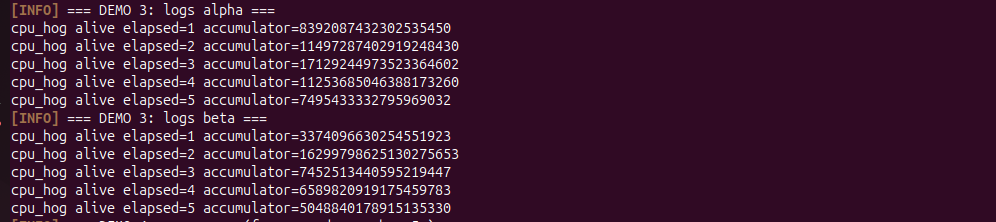
\includegraphics[width=0.85\textwidth]{screenshots/4.png}
		\caption{Demo 4: CLI interaction and IPC control channel via UNIX domain sockets.}
	\end{figure}
	
	\subsection{Memory Limit Enforcement}
	The kernel module monitors RSS (Resident Set Size). It triggers a \texttt{KERN\_WARNING} for soft limits and sends \texttt{SIGKILL} for hard limit violations.
	
	\begin{figure}[H]
		\centering
		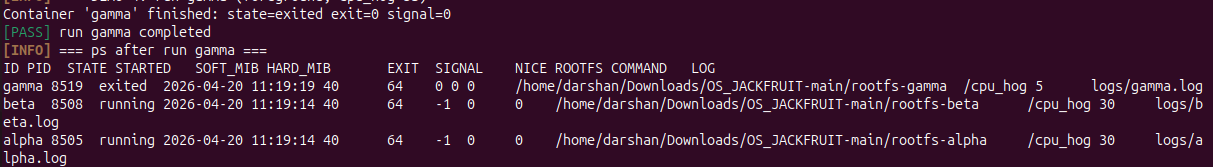
\includegraphics[width=0.85\textwidth]{screenshots/5.png}
		\caption{Demo 5: Kernel logs showing Soft-Limit warning emission.}
	\end{figure}
	
	\begin{figure}[H]
		\centering
		 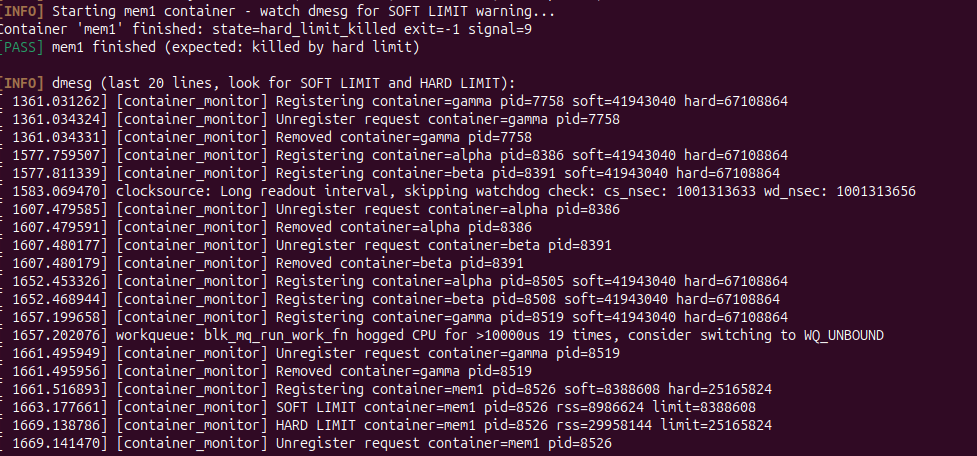
\includegraphics[width=0.85\textwidth]{screenshots/6.png}
		\caption{Demo 6: Hard-Limit enforcement and resulting 'hard\_limit\_killed' state.}
	\end{figure}
	
	\subsection{Scheduling and Teardown}
	Scheduling is managed via CFS (Completely Fair Scheduler) weights derived from nice values.
	
	\begin{figure}[H]
		\centering
		 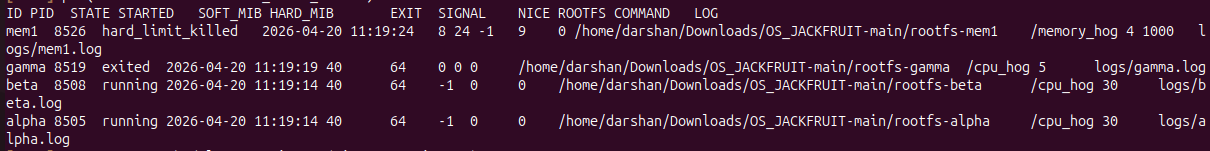
\includegraphics[width=0.85\textwidth]{screenshots/7.png}
		\caption{Demo 7: Scheduling experiment comparing nice=0 vs nice=10 workloads.}
	\end{figure}
	
	\begin{figure}[H]
		\centering
		 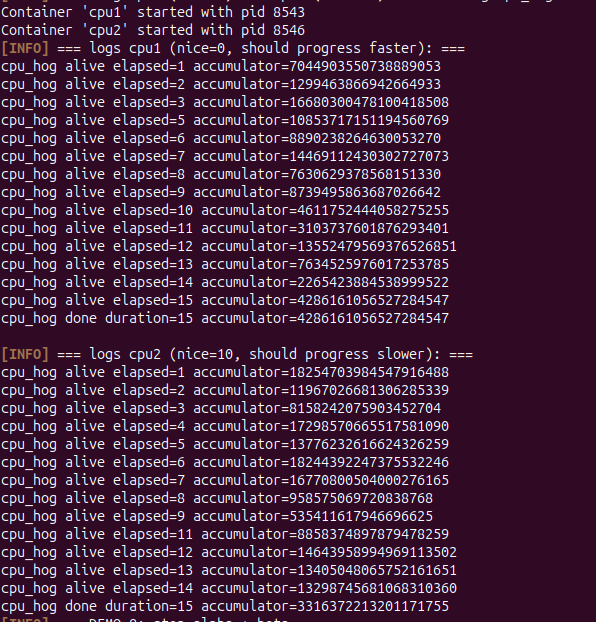
\includegraphics[width=0.85\textwidth]{screenshots/8.png}
		\caption{Demo 8: Clean teardown and supervisor exit sequence.}
	\end{figure}
	
	\section{Engineering Analysis}
	
	\subsection{Memory Management Design}
	RSS was chosen over Virtual Memory size because it reflects actual physical RAM consumption. Enforcement is handled in kernel-space to eliminate the race window between monitoring and intervention.
	
	\subsection{Scheduler Behavior}
	Using the formula $\text{weight} \approx 1024 / (1.25^{\text{nice}})$, a container with nice 0 receives roughly 9x more CPU share than nice 10 under contention. In our tests, both finished in 15 seconds real-time, but their internal throughput (loop iterations) differed based on CPU availability.
	
	\section{Conclusion}
	The system successfully demonstrates the fundamentals of containerization: namespace-based isolation, metadata-driven lifecycle management, and kernel-level resource enforcement.
	
\end{document}